\documentclass[border=10pt]{standalone}
\usepackage{pgfplots}
\pgfplotsset{compat=1.18}
\begin{document}
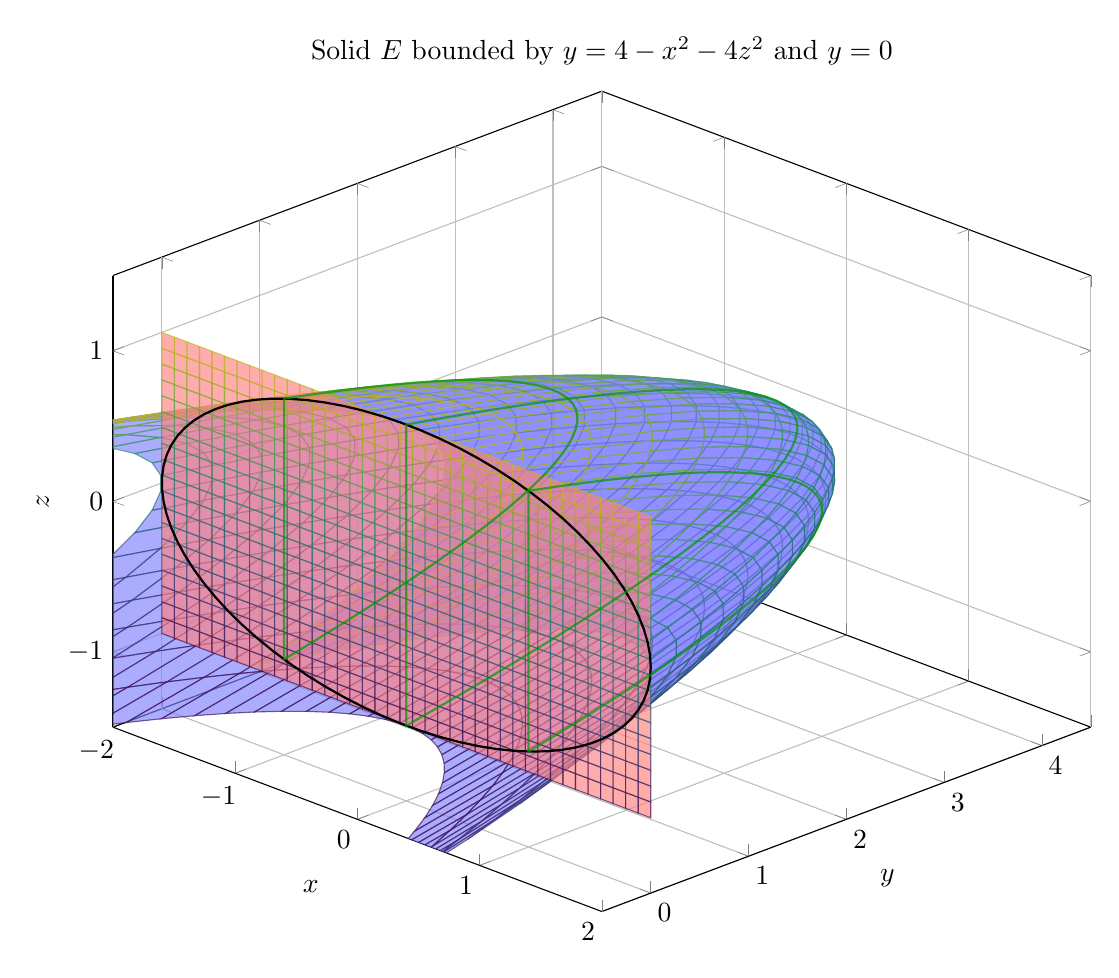
\begin{tikzpicture}
\begin{axis}[
    title={Solid $E$ bounded by $y = 4 - x^2 - 4z^2$ and $y = 0$},
    xlabel={$x$}, ylabel={$y$}, zlabel={$z$},
    xmin=-2, xmax=2,
    ymin=-0.5, ymax=4.5,
    zmin=-1.5, zmax=1.5,
    view={45}{30},
    grid=both,
    width=14cm, height=12cm,
    colormap/viridis
]

% Parabolic cylinder y = 4 - x^2 - 4z^2 (upper surface)
\addplot3[
    surf,
    domain=-2:2, samples=40,
    y domain=-1:1, samples y=20,
    z buffer=sort,
    opacity=0.65,
    color=blue!50
] ({x}, {4 - x^2 - 4*y^2}, {y});

% Plane y = 0 (lower surface)
\addplot3[
    surf,
    domain=-2:2, samples=40,
    y domain=-1:1, samples y=20,
    z buffer=sort,
    opacity=0.65,
    color=red!50
] ({x}, {0}, {y});

% Boundary ellipse at y = 0
\addplot3[
    domain=0:2*pi, samples=80,
    thick, black
] ({2*cos(deg(x))}, {0}, {sin(deg(x))});

% Cross sections at x = -1, 0, 1
\addplot3[
    domain=-1:1, samples=40,
    thick, green!60!black, opacity=0.7
] ({0}, {4 - 4*x^2}, {x});

\addplot3[
    domain=-0.866:0.866, samples=40,
    thick, green!60!black, opacity=0.7
] ({1}, {4 - 1 - 4*x^2}, {x});

\addplot3[
    domain=-0.866:0.866, samples=40,
    thick, green!60!black, opacity=0.7
] ({-1}, {4 - 1 - 4*x^2}, {x});

\end{axis}
\end{tikzpicture}
\end{document}